% This work is licensed under the Creative Commons Attribution-NonCommercial-ShareAlike 4.0 International License. To view a copy of this license, visit http://creativecommons.org/licenses/by-nc-sa/4.0/ or send a letter to Creative Commons, PO Box 1866, Mountain View, CA 94042, USA.

% language options: dutch and english - put in tips and tricks
% pass msc for master thesis and bsc for bachelor thesis
% page options: oneside for digital version, twoside for print version
\documentclass[english, msc, oneside]{layout/observatory-thesis}

\usepackage{lipsum} % only need this for the text example
\usepackage{blindtext} % only need for text example


%%%%%%%%%%%%%%%%%%%%%%%%%%%%%%%
%% Load acronyms and symbols %%
%%%%%%%%%%%%%%%%%%%%%%%%%%%%%%%

%\makeglossaries
%%%%%%%%%%%%%%%%%%%%%%%%%
%% Add custom commands %%
%%%%%%%%%%%%%%%%%%%%%%%%%
\newcommand{\tsub}{\textsubscript}
\newcommand{\tsup}{\textsuperscript}

%%%%%%%%%%%%%%%%%%%%%%%%%%%%%%%%%%%%%%%%%%%%%%%%%%%
%% Add custom units (symbols) to siunitx package %%
%%%%%%%%%%%%%%%%%%%%%%%%%%%%%%%%%%%%%%%%%%%%%%%%%%%
\def\QQ#1#2{\frac{\partial^2 #1}{\partial #2^2}}
% double partial derivative

%%%% PHYSICS / GENERAL %%%%
\DeclareSIUnit\rad{\ensuremath{\mathrm{rad}}}
\DeclareSIUnit\elementarycharge{\ensuremath{e}}                     % redefine deprecated unit
\DeclareSIUnit\clight{\text {\ensuremath {c}}_{0}}                  % redefine deprecated unit
\DeclareSIUnit\electronmass{\text {\ensuremath {m}}_{\mathrm {e}}}  % redefine deprecated unit
%%%% ASTRONOMY %%%%
%\DeclareSIUnit\angstrom{\ensuremath{\textup{\AA}}}
\DeclareSIUnit\angstrom{\ensuremath{ \mathrm{{\AA}}}}
\DeclareSIUnit\parsec{\ensuremath{\mathrm{pc}}}
\DeclareSIUnit\au{\ensuremath{\mathrm{AU}}}
\DeclareSIUnit\mas{\ensuremath{\mathrm{mas}}}

%% Sun %%
\DeclareSIUnit\msun{{M\ensuremath{_\odot}}}
\DeclareSIUnit\rsun{{R\ensuremath{_\odot}}}
\DeclareSIUnit\lsun{{L\ensuremath{_\odot}}}


%% Earth %%
\DeclareSIUnit\mearth{{M\ensuremath{_\oplus}}}
\DeclareSIUnit\rearth{{R\ensuremath{_\oplus}}}
\DeclareSIUnit\learth{{L\ensuremath{_\oplus}}}

%% Jupiter %%
\DeclareSIUnit\mjup{{M\ensuremath{_\mathrm{J}}}}
\DeclareSIUnit\rjup{{R\ensuremath{_\mathrm{J}}}}
\DeclareSIUnit\ljup{{L\ensuremath{_\mathrm{J}}}} % load custom defined units -add to tips and tricks
%%%%%%%%%%%ACRONYMS%%%%%%%%%%%%%
%\newacronym{•}{•}{•}
%To print long name of acronym again use \glsreset{acronym}

%\newacronym{acronym_reference}{acronym}{long name}

\newacronym{asteca}{ASteCA}{Automated Stellar Cluster Analysis}
\newacronym[shortplural=COM, longplural=centers of mass]{com}{COM}{center of mass}
\newacronym{gc}{GC}{globular cluster}
\newacronym{pal5}{Pal 5}{Palomar 5}
\newacronym{m5}{M5}{Messier 5}
\newacronym{m6}{M6}{Messier 6, also known as the Butterfy Cluster}
\newacronym{m31}{M31}{Messier 31, also known as the Andromeda Galaxy}
\newacronym{pca}{PCA}{principal component analysis}
\newacronym[shortplural=HR-diagrams, longplural=Hertzsprung-Russelldiagrams]{hr}{HR-diagrams}{Hertzsprung-Russelldiagram}
\newacronym{vlt}{VLT}{Very Large Telescope}
\newacronym{vlbi}{VLBI}{very-long-baseline interferometry}
\newacronym{lsst}{LSST}{Legacy Survey of Space and Time}
\newacronym{hst}{HST}{Hubble Space Telescope}
\newacronym{alma}{ALMA}{Atacama Large Millimeter Array}
\newacronym[shortplural=AGN, longplural=active galactic nuclei]{agn}{AGN}{active galactic nucleus}
\newacronym{ska}{SKA}{Square Kilometre Array}
\newacronym{2mass}{2MASS}{Two-Micron All Sky Survey}
\newacronym{cmb}{CMB}{cosmic microwave background}
\newacronym{mw}{MW}{Milky Way}
%%%%%%%%%%%%%%%%%%%%%%%%%%%%%%%%%%
%%%%%%%%%%%CONSTANTS%%%%%%%%%%%%%
\renewcommand{\glslongextraSymbolAlign}{l}

%% Important note: symbol = unit
%% Add constants to list of constants %%

%% PHYSICS / GENERAL
\glsxtrnewsymbol
    [type=constants,
    description={gravitational constant},
    symbol={\si{\num{6.674e-11}\unit{m^3.kg^{-1}.s^{-2}}}}]
    {c:G}% label (and sort valuei)
    {\ensuremath{G}}% symbol
    
\glsxtrnewsymbol
    [type=constants,
    description={speed of light},
    symbol={\si{\num{2.998e8}\unit{m.s^{-1}}}}]
    {c:c}% label (and sort value)
    {\ensuremath{c}}% symbol
    
\glsxtrnewsymbol
    [type=constants,
    description={constant of Stefan-Boltzmann},
    symbol={\si{\num{5.670e-8}\unit{W.m^{-2}.K^{-4}}}}]
    {c:sigmaSF}% label (and sort value)
    {\ensuremath{\sigma_{SB}}}% symbol
    
\glsxtrnewsymbol
    [type=constants,
    description={constant of Plack},
    symbol={\si{\num{6.626e-34}\unit{J.Hz^{-1}}}}]
    {c:plack}% label (and sort value)
    {\ensuremath{h}}% symbol

\glsxtrnewsymbol
    [type=constants,
    description={constant of Boltzmann},
    symbol={\si{\num{1.381e-23}\unit{J.K^{-1}}}}]
    {c:boltzmann}% label (and sort value)
    {\ensuremath{k}}% symbol
    
\glsxtrnewsymbol
    [type=constants,
    description={atomic mass unit},
    symbol={\si{\num{1.661e-27}\unit{kg}}}]
    {c:m0}% label (and sort value)
    {\ensuremath{m_0}}% symbol
    
\glsxtrnewsymbol
    [type=constants,
    description={rest mass of a proton},
    symbol={\si{\num{1.673e-27}\unit{kg}}}]
    {c:mp}% label (and sort value)
    {\ensuremath{m_p}}% symbol

\glsxtrnewsymbol
    [type=constants,
    description={rest mass of an electron},
    symbol={\si{\num{9.109e-31}\unit{kg}}}]
    {c:me}% label (and sort value)
    {\si\electronmass}% symbol

\glsxtrnewsymbol
    [type=constants,
    description={elementary charge},
    symbol={\si{\num{1.602e-19}\unit{C}}}]
    {c:e}% label (and sort value)
    {\si\elementarycharge}% symbol

\glsxtrnewsymbol
    [type=constants,
    description={vacuum permittivity},
    symbol={\si{\num{8.854e-12}\unit{C^2.kg^{-1}.s^2}}}]
    {c:eps0}% label (and sort value)
    {\ensuremath{\epsilon_0}}% symbol

\glsxtrnewsymbol
    [type=constants,
    description={Thomson crossection of an electron},
    symbol={\si{\num{6.652e-29}\unit{m^2}}}]
    {c:sigmaT}% label (and sort value)
    {\ensuremath{\sigma_e}}% symbol
    
\glsxtrnewsymbol
    [type=constants,
    description={gas constant},
    symbol={\si{\num{8.314}\unit{J.K^{-1}.mol}}}]
    {c:Rgas}% label (and sort value)
    {\ensuremath{R}}% symbol

\glsxtrnewsymbol
    [type=constants,
    description={constant of Avogadro},
    symbol={\si{\num{6.022e23}\unit{mol^{-1}}}}]
    {c:NA}% label (and sort value)
    {\ensuremath{N_A}}% symbol
    
%% ASTRONOMY
\glsxtrnewsymbol
    [type=constants,
    description={absolute visual magnitude of the sun},
    symbol={\si{\num{4.83}}}]
    {c:Mvsun}% label (and sort value)
    {\ensuremath{M_{V \odot}}}% symbol

\glsxtrnewsymbol
    [type=constants,
    description={apparent visual magnitude of the sun},
    symbol={\si{\num{-26.75}}}]
    {c:mvsun}% label (and sort value)
    {\ensuremath{m_{V \odot}}}% symbol

\glsxtrnewsymbol
    [type=constants,
    description={absolute B-band magnitude of the sun},
    symbol={\si{\num{5.48}}}]
    {c:Mbsun}% label (and sort value)
    {\ensuremath{M_{B \odot}}}% symbol
    
\glsxtrnewsymbol
    [type=constants,
    description={effective temperature of the sun},
    symbol={\si{\num{5778}\unit{K}}}]
    {c:Tsun}% label (and sort value)
    {\ensuremath{T_{\odot}}}% symbol

%%%%%%%%%%%UNITS%%%%%%%%%%%%%
\renewcommand{\glslongextraSymbolAlign}{l}

%% Important note: symbol = unit
%% Add units to list of units %%

% test with using \si command inside symbol environment


\glsxtrnewsymbol
    [type=units,
    description={specific intensity},
    symbol={\si{\unit{J.s^{-1}.Hz^{-1}.m^{-2}.sr^{-1}}}}]
    {u:specradiancehz} % label (and sort value)
    {\ensuremath{\mathrm{I}_\nu}} % symbol
  
\glsxtrnewsymbol
    [type=units,
    description={specific intensity},
    symbol={\si{\unit{J.s^{-1}m^{-3}.sr^{-1}}}}]
    {u:specradiance} % label (and sort value)
    {\ensuremath{\mathrm{I}_\lambda}} % symbol  
  
\glsxtrnewsymbol
    [type=units,
    description={intensity},
    symbol={\si{\unit{J.s^{-1}.m^{-2}.sr^{-1}}}}]
    {u:radiance} % label (and sort value)
    {\ensuremath{\mathrm{I}}} % symbol
    
\glsxtrnewsymbol
    [type=units,
    description={spectral flux},
    symbol={\si{\unit{J.s^{-1}.Hz^{-1}.m^{-2}}}}]
    {u:specfluxhz} % label (and sort value)
    {\ensuremath{\mathrm{F}_\nu}} % symbol    

\glsxtrnewsymbol
    [type=units,
    description={spectral flux},
    symbol={\si{\unit{J.s^{-1}.m^{-3}}}}]
    {u:specflux} % label (and sort value)
    {\ensuremath{\mathrm{F}_\lambda}} % symbol   

\glsxtrnewsymbol
    [type=units,
    description={flux},
    symbol={\si{\unit{J.s^{-1}.m^{-2}}}}]
    {u:flux} % label (and sort value)
    {\ensuremath{\mathrm{F}}} % symbol    

\glsxtrnewsymbol
    [type=units,
    description={luminosity},
    symbol={\si{\unit{J.s^{-1}}}}]
    {u:lum} % label (and sort value)
    {\ensuremath{\mathrm{L}}} % symbol    

\glsxtrnewsymbol
    [type=units,
    description={\r{A}ngstr\"{o}m},
    symbol={\si{\num{e-10}\unit{m}}}]
    {u:angstrom} % label (and sort value)
    {\si\angstrom} % symbol
    
\glsxtrnewsymbol
    [type=units,
    description={parsec},
    symbol={\si{\num{3.086e16}\unit{m}}}]
    {u:parsec} % label (and sort value)
    {\si\parsec} % symbol
    
\glsxtrnewsymbol
    [type=units,
    description={astronomical unit},
    symbol={\si{\num{1.496e11}\unit{m}}}]
    {u:au} % label (and sort value)
    {\si\au} % symbol

\glsxtrnewsymbol
    [type=units,
    description={opacity},
    symbol={\si{\unit{m^2.kg^{-1}}}}]
    {u:opacity} % label (and sort value)
    {\ensuremath{\kappa}}% symbol

%% SOLAR UNITS
\glsxtrnewsymbol
    [type=units,
    description={solar mass},
    symbol={\si{\num{1.988e30}\unit{kg}}}]
    {u:msun} % label (and sort value)
    {\si\msun}
  
\glsxtrnewsymbol
    [type=units,
    description={solar radius},
    symbol={\si{\num{6.957e8}\unit{m}}}]
    {u:rsun} % label (and sort value)
    {\si\rsun}

\glsxtrnewsymbol
    [type=units,
    description={solar luminosity},
    symbol={\si{\num{3.828e26}\unit{J.s^{-1}}}}]
    {u:lsun} % label (and sort value)
    {\si\lsun}
 
%% EARTH UNITS
\glsxtrnewsymbol
    [type=units,
    description={Earth mass},
    symbol={\si{\num{5.972e24}\unit{kg}}}]
    {u:mearth} % label (and sort value)
    {\si\mearth}
  
\glsxtrnewsymbol
    [type=units,
    description={Earth radius},
    symbol={\si{\num{6.378e6}\unit{m}}}]
    {u:rearth} % label (and sort value)
    {\si\rearth}

%% JUPITER UNITS
\glsxtrnewsymbol
    [type=units,
    description={Jupiter mass},
    symbol={\si{\num{1.898e27}\unit{kg}}}]
    {u:mjup} % label (and sort value)
    {\si\mjup}
  
\glsxtrnewsymbol
    [type=units,
    description={Jupiter radius},
    symbol={\si{\num{7.149e7}\unit{m}}}]
    {u:rjup} % label (and sort value)
    {\si\rjup}  
    
\glsxtrnewsymbol
    [type=units,
    description={arcsecond},
    symbol={\si{\frac{1}{3600}\unit{\degree}}}]
    {u:arcsecond} % label (and sort value)
    {\si\arcsecond}

\glsxtrnewsymbol
    [type=units,
    description={arcminute},
    symbol={\si{\frac{1}{60}\unit{\degree}}}]
    {u:arcminute} % label (and sort value)
    {\si\arcminute}

\glsxtrnewsymbol
    [type=units,
    description={milliarcsecond},
    symbol={\si{\num{0.001}\unit{\arcsecond}}}]
    {u:mas} % label (and sort value)
    {\si\mas}

\glsxtrnewsymbol
    [type=units,
    description={billion years (gigayear)},
    symbol={\si{\num{1e9}\unit{year}}}]
    {u:gyr} % label (and sort value)
    {\ensuremath{\mathrm{Gyr}}}

\glsxtrnewsymbol
    [type=units,
    description={electronvolt},
    symbol={\si{\num{1.602e-19}\unit{\joule}}}]
    {u:ev} % label (and sort value)
    {\si\electronvolt}

\glsxtrnewsymbol
    [type=units,
    description={density},
    symbol={\si{}\unit{kg.m^{-3}}}]
    {u:dichtheid} % label (and sort value)
    {\ensuremath{\rho}}
\makeglossaries


%%%%%%%%%%%%%%%%%%%%%%%%%%%
%% Start of the document %%
%%%%%%%%%%%%%%%%%%%%%%%%%%%

\begin{document}


%%%%%%%%%%%%%%%%%%%%%%%
%% Define parameters %%
%%%%%%%%%%%%%%%%%%%%%%%

\title{An algorithm to find dark matter wakes in galaxy simulations}
\subtitle{With a matching catchy subtitle} % optional, comment this line if not applicable
\subject{\thesistypeshort thesis} % optional, comment this line if not applicable
\author{Stephanie Carolina Cely Rodriguez}
\studentid{1013659975}
\supervisor{Dr. Veronica Arias Callejas}
\secondsupervisor{Dr. Nicolas Garavito Camargo} % optional, comment this line if not applicable
\corrector{ n}
\projectstart{Month 2022}
\projectend{Month 2023}
\affiliation{Physics deparment, Universidad Nacional de Colombia}
\address{P.O. Box 9513, 2300 RA Leiden, The Netherlands}
\coverimage{layout/figures/free_frontpage/night-sky_Evgeni_Tcherkasski.jpg}
\covercredit{Night sky by Evgeni Tcherkasski} % Note that for all the images in layout/figures/free_frontpage no credit or reference is required, but I recommend giving credit regardless.

% You can overwrite the logo with any of the UL versions in the leidenuniv_logos folder
%\affiliationlogo{layout/figures/leidenuniv_logos/Observatory_diapositive.pdf}


%%%%%%%%%%%%%%%%%
%% Frontmatter %%
%%%%%%%%%%%%%%%%%

\frontmatter % uses roman page numbering and 'frontmatter' style

\makecover % Create cover page
\maketitle % Create titlepage

% Frontmatter contents
\chapter{Abstract}

This is chapter is reserved for an abstract. \\

\noindent
% \Blindtext[1][2]
\chapter{Acknowledgements}

This is chapter is reserved for acknowledgements. \\

\noindent
\Blindtext[2][1]
\tableofcontents
\listoftables
\listoffigures
% Put acronyms, units and constants in 1 chapter

\chapter{Nomenclature}
\label{front:nomenclature}

% print acronyms (only the ones that are refered to in the text)
\printglossary[type=acronym, style=long-name-desc-loc]

\renewcommand*{\glsgroupskip}{} % no vertical indent for each new group, doesnt seem to work, hence all constants start with c: and all units start with u:

\printglossary[type=constants, style=long-name-desc-sym] % adding constants is optional
\printglossary[type=units, style=long-name-desc-sym] % adding units is optional

% Add all constants and units to the tables
\glsaddall[types=constants] % optional
\glsaddall[types=units] % optional


%\cleardoublepage

%%%%%%%%%%%%%%%%
%% Mainmatter %%
%%%%%%%%%%%%%%%%

\mainmatter % initiates arabic page numbering and 'mainmatter' style

% Input chapters
%%%%%%%%%%%%%%%%%%%%%%%%%%%%%
%% Chapter 1: The template %%
%%%%%%%%%%%%%%%%%%%%%%%%%%%%%

\chapter{The template}
\label{chap:template}
This template can be used to write your thesis. The colorpalette used in this template is built around the blue of the Leiden University logo (Lei-blauw). The colors in the palette are shown in \cref{fig:template}.

\begin{figure}[!h]
	\centering
	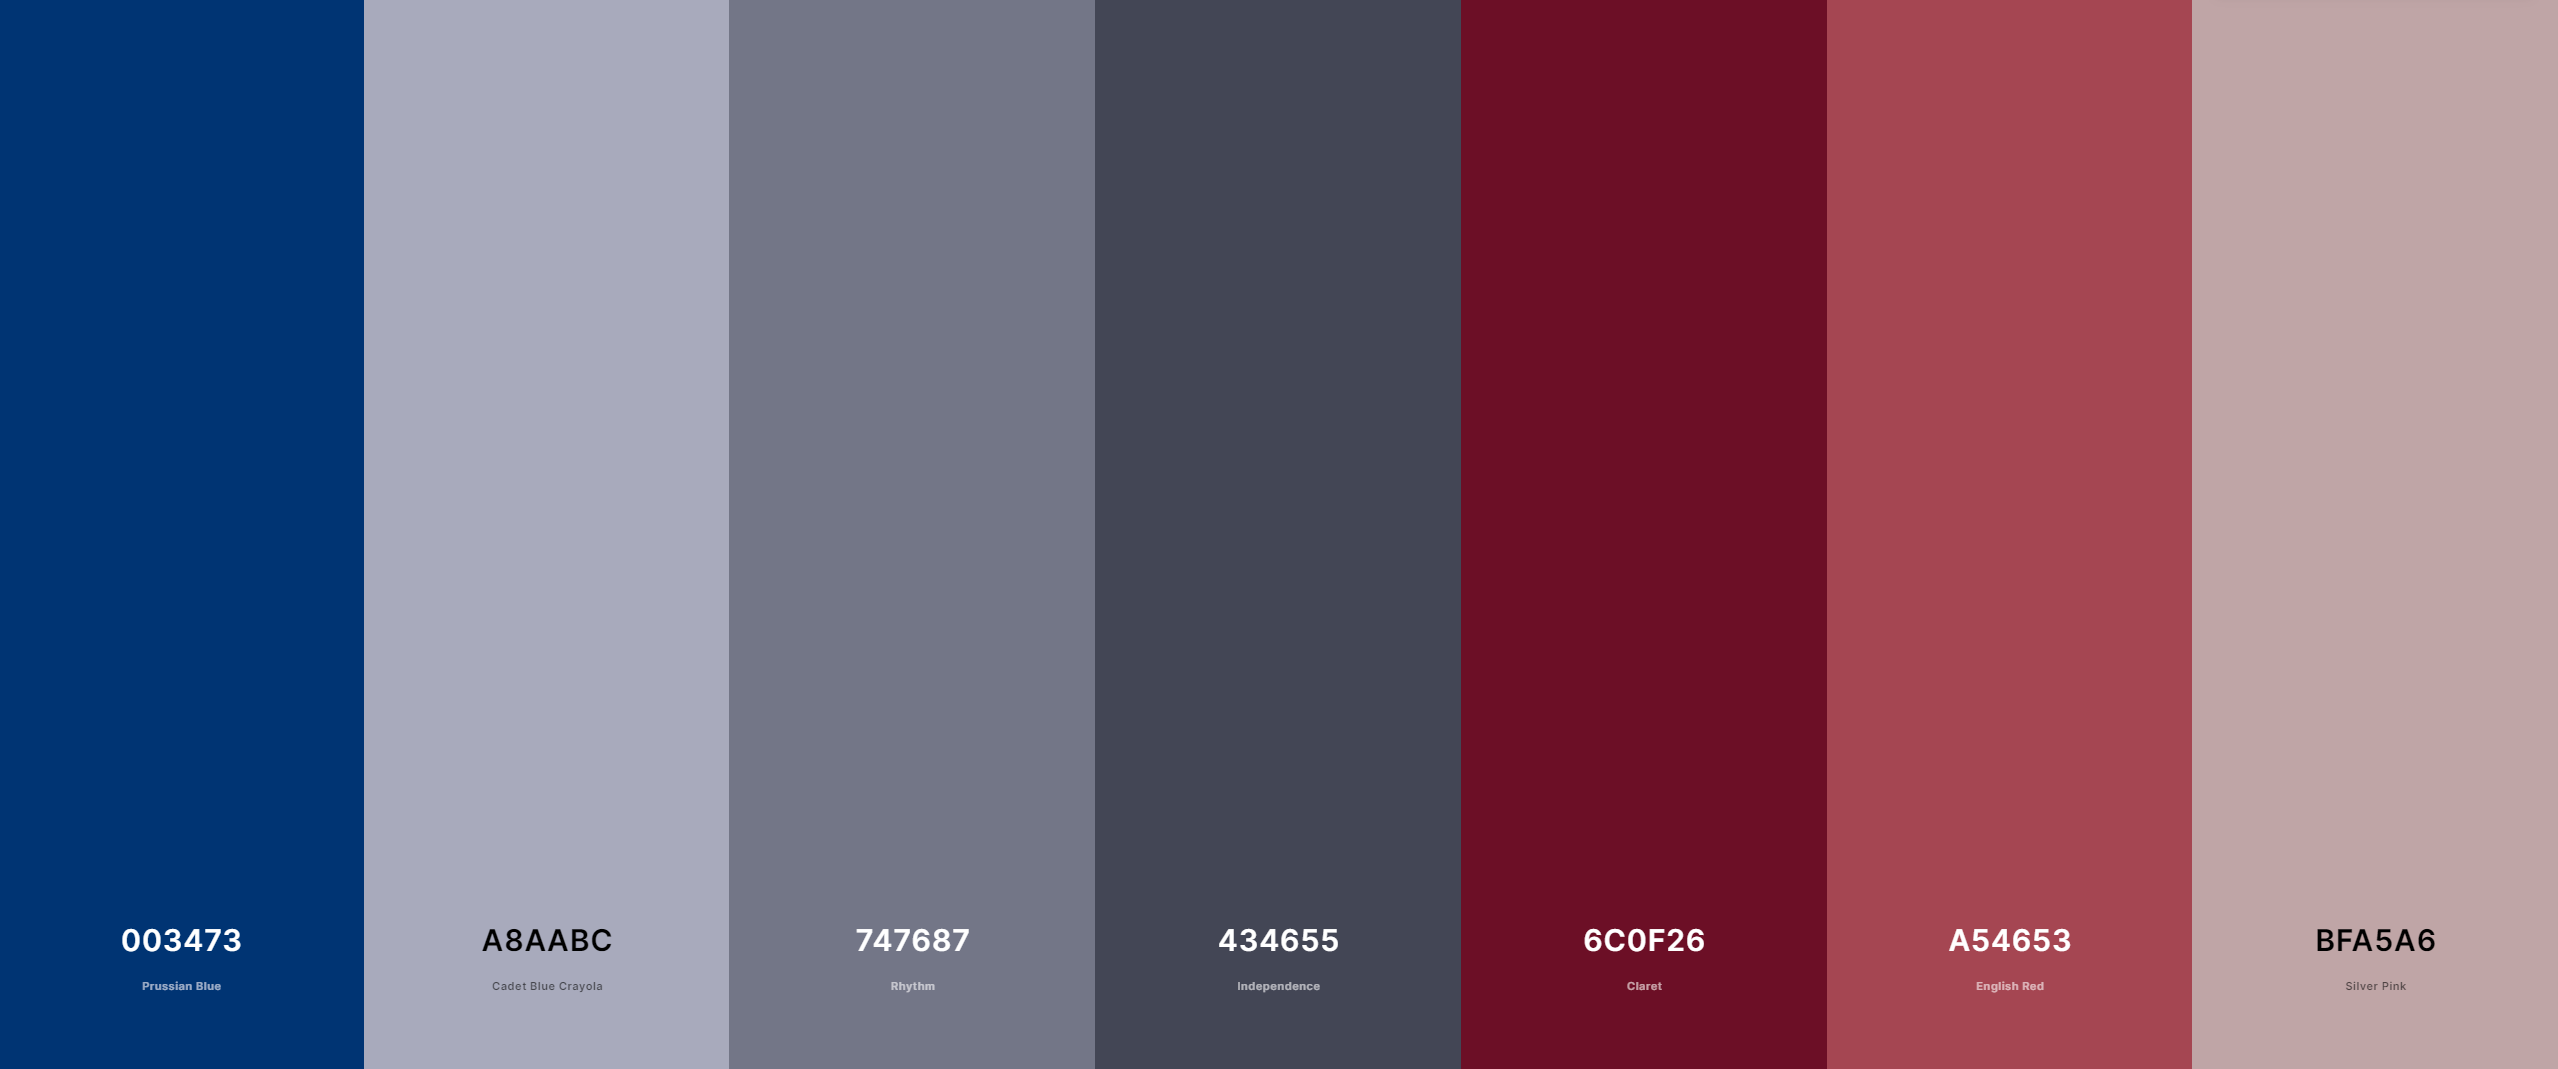
\includegraphics[width=\textwidth]{layout/figures/palette.PNG}
	\caption[Colorpalette (short caption)]{Colorpalette used in this template. Colorcodes are in hex format (HTML).}
	\label{fig:template}
\end{figure}
\noindent
\Cref{chap:tips} contains some useful tips and tricks on how to use this template and all its features. Most of these features are showcased in \cref{chap:showcase}. A Python script is included in \cref{app:script}.


%%%%%%%%%%%%%%%%%%%%%%%%%%%%%%%%
%% Chapter 1: Tips and Tricks %%
%%%%%%%%%%%%%%%%%%%%%%%%%%%%%%%%

\chapter{Tips and tricks}
\label{chap:tips}
This chapter contains some tips and tricks for using this template. \Cref{sec:tips_template} contains tips and tricks specific to this template, and \cref{sec:tips_packages} contains useful info on some of the packages used by this template.
\section{Template}
\label{sec:tips_template}
\begin{itemize}
    \item At the top of the \textit{thesis.tex} file you can change the language passed to \textit{documentclass}. When changing this to Dutch, the nomenclature titles and Leiden University logos will also be changed to the Dutch versions.
    \item For a bachelor thesis, pass bsc instead of msc to \textit{documentclass}.
    \item You can change parameters such as author, supervisors and coverimage right after the start of the document in \textit{thesis.tex}.
    \item The logo's are defined in \textit{layout/observatory-thesis.cls}, with \textbackslash coveraffiliationlogo  for the logo on the coverpage, and \textbackslash affiliationlogo for the logo on the titlepage. Note that the current logo on the coverpage is the diapositive version; if your coverimage is lighter, use the normal logo instead.
    \item Folder \textit{layout/figures/free\_frontpage} contains some other free frontpage images that don't require credit (although I do advocate giving credit regardless). You can remove unused images to save space.
    \item There are additional caption settings available. When defining a caption, you can use \textbackslash caption[short caption]\{long caption\}. The short caption will be listed in the list of figures or list of tables at the start of the document, and the long caption will be shown below the figure or above the table. Use \textbackslash imref\{\} to add an image credit entry below the caption, as shown in \cref{fig:prettypicture} and \cref{fig:NGC1300}.
    \item If you want to print your thesis, you can pass \textit{twoside} instead of \textit{oneside} to \textit{documentclass} in \textit{thesis.tex}. This will make the inner margin bigger than the outer margin, ensure all chapters start at the left page, and display the chapter title at the top of the left page and the section title at the top of the right page.
    \item If you input chapters (or even sections) separately, you can comment out the \textit{\textbackslash include} of the chapters you are currently not editing to make the document compile faster.
    \item This template uses the AASTeX bibliography style, see \cref{sec:acr_refs} for examples of citations. All journal abbreviations used in the ADS BibTeX entries are defined at the bottom of the class file. Examples are \textit{\textbackslash aap} ( \aap) and \textit{\textbackslash aap} ( \apj).
    \item The included bibliography, \textit{bib.bib}, shows more (uncited) examples of sources, such as conference proceedings and unpublished work.
    \item When you get errors after adding a new entry in your bibliography, it is most commonly caused by a special character in a name, for example é and ö. You can fix this by replacing the character with the corresponding latex encoding, in this case \textbackslash'\{e\} and \textbackslash"\{o\} respectively.
\end{itemize}

\section{Packages}
\label{sec:tips_packages}
\begin{itemize}
     \item This template includes the \texttt{\href{https://ctan.org/pkg/cleveref}{cleveref}} package, which has advantages over the the normal \textbackslash ref. The commands of this package are \textbackslash cref and \textbackslash Cref. When using this, it will automatically include the word of whatever it is you are referring to before the number (such as chapter, section, appendix, table, figure). This way you don't have to worry about manually changing all the references when you change the structure of your thesis by for example changing a chapter into a section.
    \item The package \texttt{\href{https://ctan.org/pkg/siunitx}{siunitx}} includes many useful features for displaying (scientific) numbers and units. You can also define your own custom units; some astronomy units have already been added in \textit{glossaries/custom\_units.tex}.
    \item This template uses the packages \texttt{\href{https://ctan.org/pkg/glossaries}{glossaries}} and \texttt{\href{https://ctan.org/pkg/glossaries-extra}{glossaries-extra}}. It is set up such that it automatically creates a table with acronyms, constants and units. You can find these after the list of figures and list of tables. You can see how the acronyms, constants and units are defined in  \textit{glossaries/acronyms.tex}, \textit{glossaries/units.tex} and \textit{glossaries/constants.tex} respectively, such that you can add new ones yourself. \Cref{sec:acr_refs} shows various ways to use the acronyms in your text. All of these are clickable and will take you to the corresponding table at the start of the document.
    \item You don't want acronyms in titles or in captions to be clickable. Always use \textbackslash glsfmtshort and \textbackslash glsfmtlong for the acronym and the full word respectively.
    \item This class includes package \texttt{adjustbox}, which allows figures to float outside the page margins whilst remaining centered. Although for aesthetics it is not recommended to do this, if you see no other way to include your figure in a clearly readable way, you can make it exceed the margins by using: \textit{\textbackslash includegraphics[width=1.2\textbackslash textwidth, center]\{figures/figuretitle.png\}}
\end{itemize}

%%%%%%%%%%%%%%%%%%%%%%%%%
%% Chapter 2: Showcase %%
%%%%%%%%%%%%%%%%%%%%%%%%%

\chapter{Showcase}
\label{chap:showcase}
\Cref{sec:acr_refs} shows examples of the usage of the package \texttt{glossaries} and of adding citations. \Cref{sec:subsection} displays what subsections look like in this template, and \cref{sec:math} showcases a large variety of math symbols and equations. The last section, \cref{sec:text}, shows a large patch of text with some (wrap)figures and table.

\section{Acronyms and references}
\label{sec:acr_refs}
Here is a nice acronym test: two big \glspl{gc} are \gls{pal5} and \gls{m5}. \Gls{m6} is an open cluster, whereas \gls{m31} is a galaxy. Here is another acronym that starts with a "p": \gls{pca}. When acronyms are referenced a second time, it only shows the short name: \gls{pal5}, \gls{m5}. One single \gls{gc}, and multiple \glspl{gc}. One \gls{agn}, multiple \glspl{agn}, and multiple long \glsxtrlongpl{agn}. This is an example of an unclickable short reference, \glsfmtshort{vlt}, an unclickable long reference, \glsfmtlong{vlbi}, and an unclickable plural form of a short reference \glsfmtshortpl{gc}. Unclickable references do not show up in the nomenclature if they are not referred to anywhere else in the text. You will see that \gls{vlbi} is listed in the nomenclature, but \glsfmtshort{vlt} is not. 

This is an example of a paragraph with in-text
citations using the aasjournal BibTeX style.
Here is a reference to a journal article with
a single author \citep{article}, to a journal
article with two authors without parenthesis \citet{article2}, and to a journal article with six authors \citep{article6}. Here is a citation to a book \citep{book}.

\section{Subsectionceptionsection}
\label{sec:subsection}
This is the first section of the subsectionceptionsection. Let's start with some text. \lipsum[66]
\subsection{Subsection of the first section}
Look, its a subsection.
\subsection{Another subsection}
And there is more!
\subsection{Third's a charm}
Welcome to the final subsection.

\section{Math}
\label{sec:math}
\def\ii{\mathrm{i}}
\def\pp{\mathrm{\pi}}

Basic examples of equations:
\begin{itemize}
\item Moment of inertia:
\begin{align}
    \sum_{i=1}^N m_i\vec{r_i}^2
\end{align}
  \item Einstein's field equations:
    \begin{align}
        G_{\alpha\beta} &\equiv R_{\alpha\beta}-\frac{1}{2} g_{\alpha\beta}R+\Lambda g_{\alpha\beta}=\frac{8\pi\kappa}{c^2}T_{\alpha\beta}
    \end{align}
\item Main-sequence relations:
    \begin{align} 
    \qquad \frac{L}{\si\lsun} &= 
    \left\{
    \begin{aligned}
     &0.35\left(\frac{M}{\si\msun}\right)^{2.62}, &M&<0.7\si\msun \\
     &1.02\left(\frac{M}{\si\msun}\right)^{3.92}, &M&\geq 0.7\si\msun
    \end{aligned}
    \right.                                                 \label{eq:mass_light} \\
        \qquad \frac{R}{\si\rsun} &= 
    \left\{
    \begin{aligned}
     &1.06\left(\frac{M}{\si\msun}\right)^{0.945}, &M&<1.66\si\msun \\
     &1.33\left(\frac{M}{\si\msun}\right)^{0.555}, &M&\geq 1.66\si\msun
    \end{aligned}
    \right.                                                 \label{eq:radius_mass} 
    \end{align} 
\item Wave functions:
\begin{align}
\Phi(k,t)&=\frac{1}{\sqrt{h}}\int\Psi(x,t){\rm e}^{-ikx}dx,  
&\Psi(x,t)&=\frac{1}{\sqrt{h}}\int\Phi(k,t){\rm e}^{ikx}dk \\
\langle f(t)\rangle &=\iiint\Psi^* f\Psi d^3V, &\langle f_p(t)\rangle &=\iiint\Phi^*f\Phi d^3V_p
\end{align}
\item Wave equation:
\begin{align}
\nabla^2u-\frac{1}{v^2}\QQ{u}{t}=\QQ{u}{x}+\QQ{u}{y}+\QQ{u}{z}-\frac{1}{v^2}\QQ{u}{t}=0
\end{align}


\end{itemize}

\section{Text and figures}
\label{sec:text}
\begin{wrapfigure}{r}{0.5\textwidth}
    \vspace{-1em}   % sometimes needed to align the image, 1 em is size of capital M, 1 ex of lower case x
	\centering
	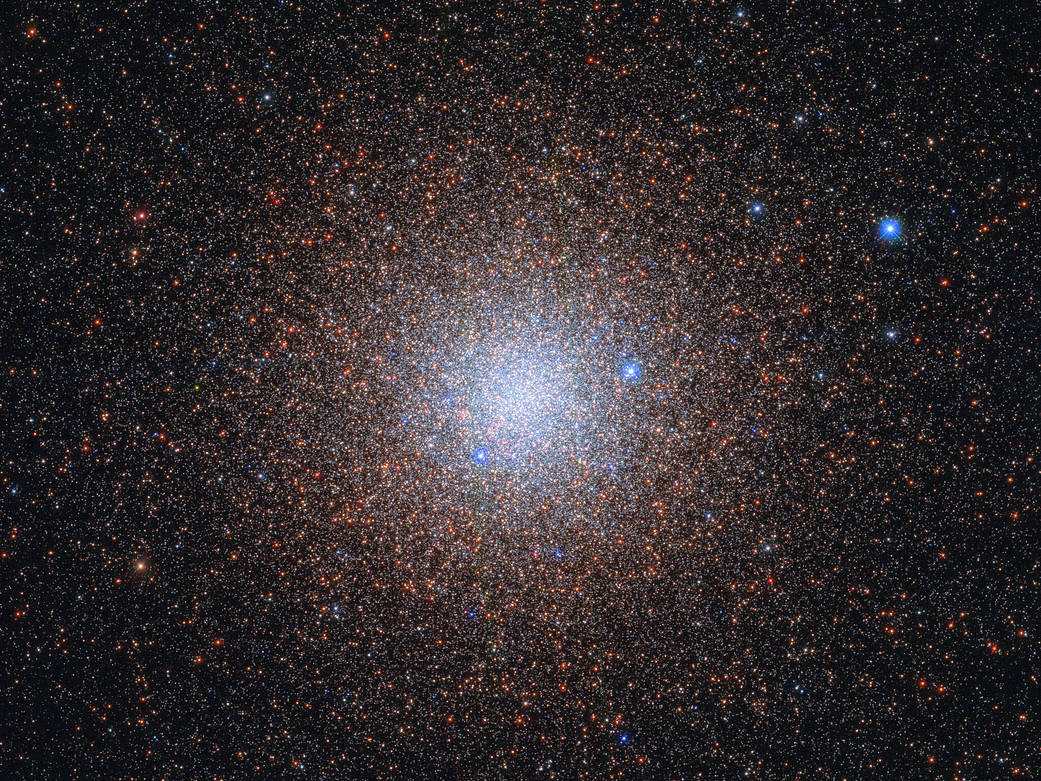
\includegraphics[width=0.5\textwidth]{figures/gc_image.jpg}
	\caption[A picture of NGC 6441.]{A picture of NGC 6441, one of the most massive and luminous GCs in the Milky Way.}
	\label{fig:prettypicture}
	\imref{Image credit: ESA/Hubble \& NASA, G. Piotto}
    %\vspace{-1ex}
\end{wrapfigure}
Check out \cref{fig:prettypicture}, \cref{fig:NGC1300} and \cref{tab:example_table}!
\lipsum[1-3]

\begin{table}[t]
    \centering
    \caption{An example table showing ranges for fundamental parameters.}
    \label{tab:example_table}
    \begin{tabular*}{\textwidth}{c @{\extracolsep{\fill}}cc}
    \hline 
    Parameter & Min & Max \\ 
    \hline \hline
    Z & 0.0001 & 0.0099  \\ 
    \hline 
    a & 9.9 & 10.29 \\
    \hline 
    E & 0 & 1 \\
    \hline 
    D & 14 & 20 \\
    \hline 
    M & 1000 & 80000 \\
    \hline 
    b & 0.0 & 0.8 \\
\hline 
\end{tabular*} 
    \subcaption*{The ranges of the metallicity (Z), the log(age) (a), the extinction (E) in B-V colour index, the distance modulus (D), the mass (M) in solar masses and the binary fraction (B).}
\end{table}

\lipsum[5-8]
\begin{figure}[b!]
	\centering
	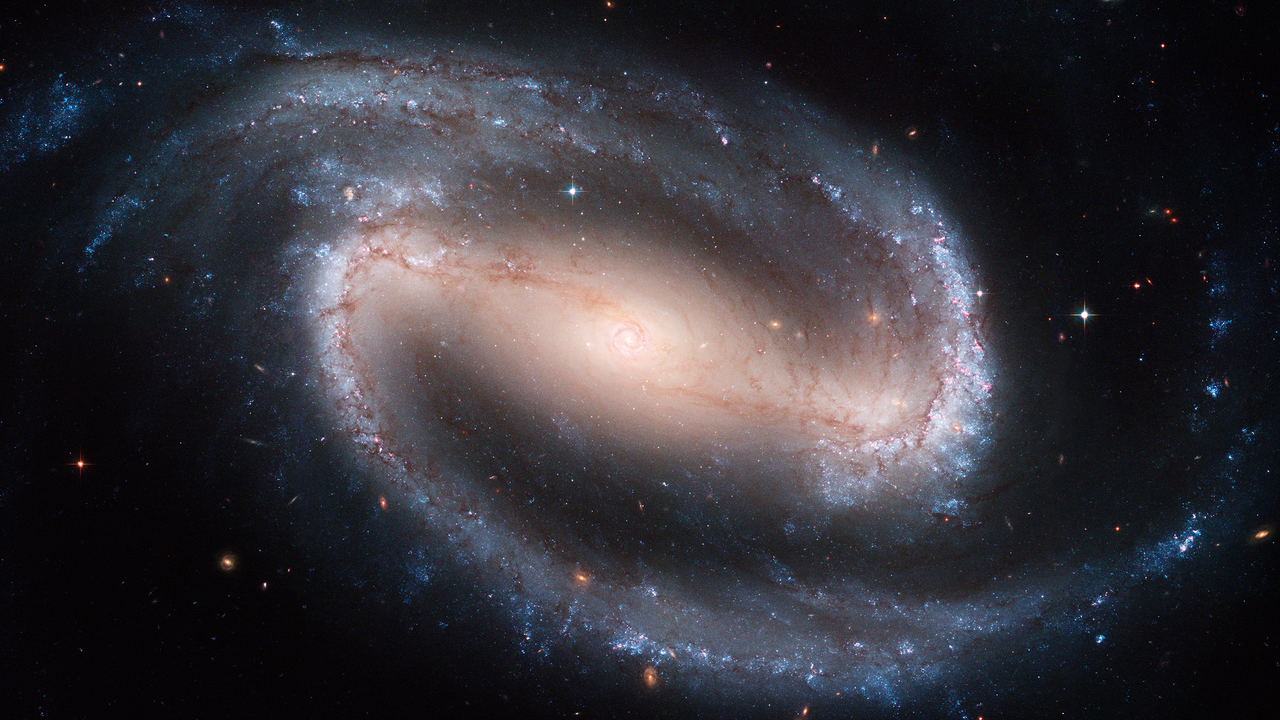
\includegraphics[width=\textwidth]{figures/NGC1300.png}
	\caption[An image of NGC 1300.]{One of the largest \glsfmtshort{hst} images ever made of a complete galaxy; an image of NGC 1300.}
	\label{fig:NGC1300}
    \imref{Credit: NASA, ESA, and The Hubble Heritage Team (STScI/AURA); \\
    Acknowledgment: P. Knezek (WIYN)}
\end{figure}
\lipsum[9-16]

Here are some more predefined acronyms to show different pages listed in the nomenclature: \gls{com}, \gls{hr}, \gls{lsst}, \gls{hst}, \gls{alma}, \gls{ska}, \gls{2mass} and \gls{cmb}.



%%%%%%%%%%%%%%
%% Appendix %%
%%%%%%%%%%%%%%

\appendix % initiate roman chapter numbering

% Appendices
\chapter{A script}
\label{app:script}

\lstinputlisting{appendix/pythonscript.py}
%\label{app:code.infoblok}

% Bibliography
\bibliographystyle{layout/aasjournal}
\bibliography{bib}
\end{document}
